% Preamble
\documentclass[a4paper,12pt]{article}

\usepackage[osf]{mathpazo} % palatino
\usepackage{ms}            % load the template
\usepackage[round]{natbib} % author-year citations
\usepackage{graphicx}      
\pagenumbering{arabic}    

% From Syst Biol template
\linespread{1.66}
\raggedright
\setlength{\parindent}{0.5in}

\pagestyle{empty}

\renewcommand{\section}[1]{
  \bigskip
  \begin{center}
  \begin{Large}
  \normalfont\scshape #1
  \medskip
  \end{Large}
  \end{center}
}

\renewcommand{\subsection}[1]{
  \bigskip
  \begin{center}
  \begin{large}
  \normalfont\itshape #1
  \end{large}
  \end{center}
}

\renewcommand{\subsubsection}[1]{%
\vspace{2ex}
\noindent
\textit{#1.}---}

\renewcommand{\tableofcontents}{}

\bibpunct{(}{)}{;}{a}{}{,}  % this is a citation format command for natbib

% Ignoring their title page setup as I like Rich's template better :)

% Title page information

\title{The ``Dark Side'' of Phylogenetic Comparative Methods}
\author{
  Richard G. FitzJohn$^{1}$, Cecile An\'{e}$^{2}$, Wayne Maddison$^{3}$,\\ Matthew W. Pennell$^{4}$, Gavin H. Thomas$^{5}$, April Wright$^{6}$,\\ and Natalie Cooper$^{7,8,*}$
}
\date{}
\affiliation{\noindent{\footnotesize
$^1$ Department of Biological Sciences, Macquarie University, Sydney, NSW 2109, Australia. \\
$^2$ Wisconsin\\
$^3$ UBC\\
$^4$ Institute for Bioinformatics and Evolutionary Studies, University
of Idaho, Moscow, ID 83844, U.S.A.\\
$^5$ Sheffield\\
$^6$ Austin\\
$^7$ School of Natural Sciences, Trinity College Dublin, Dublin 2, Ireland.\\ 
$^8$ Trinity Centre for Biodiversity Research, Trinity College Dublin, Dublin 2, Ireland.\\
$^*$ Corresponding author: ncooper@tcd.ie; Zoology Building, Trinity College Dublin, Dublin 2, Ireland. Fax: +353 1 677 8094; Tel: +353 1 896 1926.\\
}}

\vfill
%\paragraph{Word-count:} X words

\runninghead{The ``Dark Side'' of PCMs}
\keywords{PCM, assumption, etc.}

% End of preamble

\begin{document}
\modulolinenumbers[1]   % Line numbering on every line

\mstitlepage
\parindent = 1.5em
\addtolength{\parskip}{.3em}

%\section{abstract}
% If Syst Biol "Point of View" there's no abstract

\newpage
\raggedright
\doublespacing
%\section{Introduction} % No intro heading for Syst Biol

A long time ago in a galaxy far, far away - also known as the 1980s - phylogenetic comparative methods (PCMs) were developed to deal with the statistical non-independence of species in comparative analyses (e.g. \citealp{felsenstein1985phylogenies,grafen1989phylogenetic}). 
Since then PCMs have been extended to investigate evolutionary pattern and process, and include methods for investigating drivers of diversification, the tempo and mode of trait evolution, and models of speciation and extinction (see reviews in \citealp{o2012evolutionary, pennell2013integrative}). 
PCMs have also become extremely popular over recent years; the number of papers containing the phrase `phylogenetic comparative' has increased exponentially since the 1980s (Figure \ref{PCMCitations}). 
With new methods being published almost weekly, there has never been a better time to be a comparative biologist.

\begin{figure}[h]
\centering
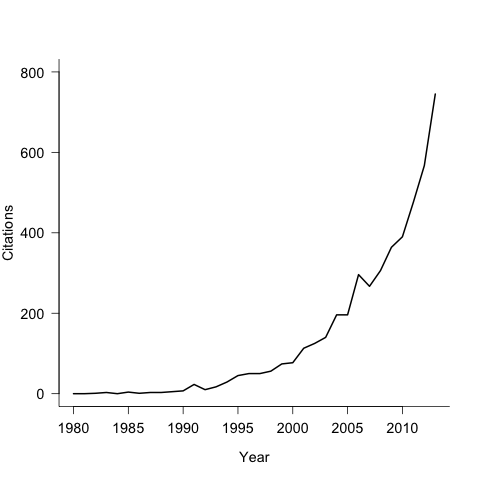
\includegraphics[width = 10cm]{PCMCitations.png}
\caption{PCM papers through time}
\label{PCMCitations}
\end{figure}

Unfortunately, PCMs also have a ``dark side''; they make various assumptions and suffer from biases in exactly the same way as any other statistical method \citep{freckleton2009seven,boettiger2012your}. 
The more popular these methods become, the less awareness methods-users seem to have of this dark side. Increasingly assumptions and biases are inadequately assessed in empirical studies, leading to poor model fits and misinterpreted results. 
Additionally, little consideration is given to whether using a PCM is really appropriate for the question at hand \citep{losos2011seeing}. 
To paraphrase \citet{blomberg2012independent}, the enthusiastic application of PCMs has greatly outpaced our theoretical understanding of the methods and their relations to the rest of statistical theory.\\

% Do we need more explicit comments showing we're not the only people to think this, nor the first to say it?

One major issue is that two groups of people are involved with PCMs. 
At one extreme, methods-developers (``wookies'') develop new methods and implement them. They are (generally) aware of the limitations of their methods, and the assumptions that underly them. 
% Bit of a stretch but we can pretend right? :)
At the other extreme, na\"{i}ve methods-users (``ewoks'') just want to use PCMs to answer empirical questions with their data, and may not be aware of issues with the methods 
%when the next sentence is not in brackets it breaks the flow. But needs to be here. Brackets feel wrong too. Will Syst Biol allow footnotes
(of course the majority of people fall somewhere between these two extremes on the ``wookie-ewok'' spectrum; many methods-developers are developing methods with a specific empirical question in mind, while there are many advanced methods-users who have detailed knowledge of the limitations of the methods they use). 
The problem is that although methods-developers (and advanced methods-users) are aware of the problems with PCMs, this information is not being effectively transferred to methods-users. 
Additionally, the tools and approaches used to fit models are often far more user-friendly and better documented than the methods used to to assess whether that model fit is reasonable. 
Clearly more effort is needed to bridge the widening gap between methods-users and methods-developers. Here we explore the causes of this communication gap and suggest some potential solutions. %still not happy with this writing

\section{What impedes information transfer from methods-developers to methods-users?}
% Or something similar

As scientists we mainly communicate our ideas through the literature. Therefore, any difficulty transferring information between methods-developers and methods-users must begin there. If this is the case we suggest three possible reasons:
%Yuk fix this

\begin{enumerate}
\item Not everything is mentioned in the literature.
\item The literature is too technical and/or important details are hidden within the text.
\item Methods-users have bypassed the literature and gone straight to the implementation of the method.
\end{enumerate}

%Note that we assume that methods-users ignore assumptions and biases because they are unaware of them. Of course, there may be methods-users who are perfectly aware of these issues but choose to sweep them under the carpet to get their work published. Although we believe there is no excuse for doing this, we also recognize that the ``publish or perish'' culture of academia may pressurize nontenured scientists into this. Hopefully some of the changes we suggest below will also help with this problem. 
%This could be a footnote, or left out!

\subsection{1. Not everything is mentioned in the literature}

A lot of the information needed to properly apply PCMs is not found in the literature. 
We refer to this knowledge as ``PCM folklore'' because it tends to be passed down from PIs to graduate students, and it is occasionally closer to fiction than fact.
Sometimes the folklore includes tricks to get methods working, or useful rules-of-thumb. 
Other times folklore is more opinion-based, but over time these opinions become rules. 
One example of such folklore is in the defaults of programs that perform PCMs. 
These often start out as arbitrary starting points for data exploration with no justification for their use, but over time become the way the analysis is always performed.
Useful PCM folklore is often shared among methods-developers, and among collaborating groups, but is rarely shared outside of these circles. 
When it is shared, it tends to be in the form of email exchanges between methods-developers and struggling methods-users.
This advice is extremely useful to the methods-user in question, but forms a kind of ``dark advice'' that isn't accessible to the rest of the community.\\

% Do we want a specific example here? Theta estimation in OU models? 
% Could mention ±3 from Jones&Purvis97 - totally unjustified rule of thumb now = canon.
% Mention hidden assumptions?

Other information about the limitations of a method may be absent from the literature due to the time lag between a new method being published and others having time to test and critique it. 
For example, Felsenstein published the phylogenetic independent contrasts method in 1985, but it wasn't until the early 1990s that real critiques of the method and its assumptions began to be published. %add citations.
This time lag is shorter with more recent methods because simulations testing the method are now required by journals.
However, we suspect there are still many hidden assumptions and biases in virtually all new PCMs that have yet to be properly explored in the literature. 
%We can cite your paper on Pagel 1994 here if you like - as an example of old methods that are still being investigated.

\subsection{2. The literature is too technical and/or important details are hidden}

Although a lot of information is not found in the literature (see above), the majority of assumptions and biases of PCMs are documented somewhere. 
A big issue for novice methods-users is that this information is often extremely technical and dense.
It is not unusual for papers to be full of equations, over 20 pages long, and written in a way that gives even advanced users a headache. 
Additionally there is a lot of literature to wade through before getting all of the required information. 
For example, one of us (NC) recently reviewed papers discussing the assumptions and limitations of the most commonly used PCM, phylogenetic independent contrasts \citep{felsenstein1985phylogenies}. 
Even with prior knowledge of the key papers and authors to focus on, this resulted in XX pages, XX papers and a book to read. 
This seems like an excessive amount of reading to expect from a methods-user trying to run a simple empirical analysis.\\

Another issue is that it can sometimes be hard to find the information required. Assumptions and caveats can be found in the Introduction, Methods, Results and/or Discussion of a paper. 
They are rarely neatly corralled in one place, making it really easy to miss pertinent details. 
This places an additional burden on methods-users who must read every paper very carefully.

\subsection{3. Users jump straight to the implementation of the method}

In the early days of PCMs, some methods-developers provided stand alone packages to run their methods, others provided code in whichever language they were comfortable programming in, and still others provided no way of implementing their methods at all. 
This resulted in many frustrating hours (and days and months!) trying to implement any new method you wanted to use.\\

More recently however, the PCM community has moved towards mostly implementing their methods in R (cite), and code sharing has become almost ubiquitous. 
The number of R packages for PCMs has increased exponentially since 2005 when APE (cite) was released, and has increased particularly sharply since 2008 (Figure \ref{x}).
Simultaneously, more and more methods-users are able to use R, thus when a new method is published they can now take an R package ``off the shelf'' and use it to run the method immediately.
This has led to an increasing number of methods-users jumping straight to the implementation of a method, without really carefully trying to understand what the method is doing, what its assumptions might be, or what the results they extract really mean in a biological context.
This problem is exacerbated by the fact that manuals, vignettes and help files for R packages rarely mention the assumptions of the method, or how to test model fit. 
The APE book (cite) for example, provides no guidance on assumption testing in its chapter on phylogenetic independent contrasts, even though the methods needed to do this are well-established and very easily implemented in R (for a counter example see CAIC and caper documentation - cite).\\
We believe this issue is probably one of the biggest currently facing phylogenetic comparative biology. It is extremely frustrating reading/reviewing papers where the authors have clearly not carefully read or understood the primary literature on the method they are using. 
Additionally, many methods-users seem to try to retrofit a question so they can use the newest shiniest methods available. This is all driven by our ``publish or perish'' culture, and the pressure to produce as many papers as possible out of a dataset.
The truly sad thing about this state of affairs is that by making science more open and sharing code (something we are all passionate about and strongly support) we seem to have made the situation worse rather than better (\citealp{freckleton2009seven}, for example, mentions R as a way of improving things). %needs a bit of finessing

\section{How can we solve some of these problems?}

%The problems described above require action by methods-developers, methods-users and the community as a whole. %Can't expect empiricists to be an expert in every method, but do want to add to workload of overloaded developers.
%Can we expect methods users to read every paper before using a method? (Yes – wouldn’t let someone work on your microscope unless you were sure they knew what they were doing!!!). 

\subsection{1. Simplify, summarize and share}

Many of the problems above are caused by methods papers being difficult to read. 
This isn't entirely the fault of methods-developers; most journals have strict word limits so it's often easier to use a one line equation rather than a paragraph of description. 
However, it's hard to complain about novice users failing to understand a method when the paper is incomprehensible. %cough cough Hansen. Ow my eyes are bleeding.
One solution is to prepare an accompanying blog post or video explaining the method in less technical terms. 
Some journals already encourage this (e.g. Methods in Ecology and Evolution), and even if they do not, there is no harm in doing this and hosting it on a personal website. 
The ability to share ideas with a non-technical audience is a key skill to develop, and it may even encourage more people to use the method. 
%Another more %knitr reports in supp mat (e.g. cite that nice paper )
At the very least, having a simple list of the main assumptions, biases and caveats of the method somewhere would reduce misuse and provide a place to point methods-users to when they begin using a method.
Of course this will be difficult as there are often hidden assumptions in a method, and listing all possible assumptions and caveats may be unfeasible.\\

%Want to mention adding ways of testing assumptions to packages
%follow up papers (hard to publish coz they are incremental - see incentives)
%or should this go in incentives...?

The glut of literature that already exists for established methods is a bigger problem. 
One solution would be to establish a wiki-style website where methods-developers and advanced methods-users could post summaries of commonly used methods, along with lists of key papers to read. 
The community would be responsible for peer reviewing these summaries to ensure all opinions are covered. 
Eric Matsen's Phylobabble discourse page (link) is an excellent example of a similar approach for phylogenetics. Unfortunately this would be hard to arrange as there is little incentive for methods-developers and advanced methods-users to contribute to such a project at the cost of time pursuing their own research.\\

One solution we believe will be of use is establishing a discourse page for providing R help. 
Currently most methods-users either email the R-sig-phylo help list or the package developer for assistance. 
Both approaches are suboptimal. 
R-sig-phylo is impossible to search effectively, leading to the same questions being dealt with repeatedly. 
The same is true in email exchanges between methods-users and package developers with the added issue of this being ``dark advice'' that isn't shared. 
A discourse page would collate all of this information and reduce pressure on package developers by allowing advanced methods-users to help novice users. 
This would be a valuable resource for methods-users and also reduce the amount of time methods-developers spend dealing with queries.
We floated this idea at Evolution 2014 and hope to have a version of the discourse page up and running soon.

\subsection{2. Read, think and learn}
%This section is currently a bit personal. You should do this and that, rather than methods-users should do this and that.
If methods-developers are going to put time and effort into making their methods easier to understand, then methods-users need to take advantage of this and work harder to understand the methods they are using. 
At a minimum, methods-users should read the original papers describing a method, and any recent updates. 
Jumping straight in to an R implementation is a fine way to start a project, but it needs to be followed up by careful reading and thought. 
Playing with shiny new methods is always fun, but don't retrofit your question to the new method. 
Think carefully about the question you want to ask, and whether the method really answers that question. 
Also consider whether you really need to use a phylogeny for your analysis at all \citep{losos2011seeing}.\\

Another key skill to develop is distrust! 
Never take results from PCMs (or any other statistical analysis) at face value. 
Always think carefully about whether there may be hidden assumptions or biases that have not been explored in the accompanying papers. 
A good way to check this is to simulate some data and see if you get the results you expect. 
Also consider whether the method will work on your dataset; how many species does it need to have reasonable power, how does it deal with polytomies, can it cope with non-ultrametric trees etc.
Finally, never be afraid to question standard practice, sometimes it's just PCM folklore
%Could add my pglm vs pgls example.

\subsection{3. Collaboration}

A obvious solution to all these problems is for methods-developers and methods-users to collaborate more. 
The benefits to methods-users are obvious, but methods-developers can also benefit by gaining extra datasets to test their ideas on and people who will discover corner cases and bugs in their software before it get released. 
A big difficulty with collaboration is that it is often asymmetrical in terms of benefit to methods-users and methods-developers. 
Methods-developers and advanced methods-users can often put a lot of time and effort into running analyses for less experienced colleagues, yet at best they come out of the experience with a middle authored paper. 
Until these author positions are considered equal to first and last author positions, there is little incentive to collaborate extensively.

\subsection{4. Incentives}

%Improvements in methods, and ways of detecting biases etc should be sufficient for publication (rather than MEE's weird focus on novelty now it has a huge IF)

%Incentives - funding for pure methods. Different authorship rules. 
%Change the definition of success in academia. Quality not quantity. Remove rush to publish. This would help WOMEN too!

%We really *do not* want to lose all the technical people from science. We need them more than ever as evo bio becomes more and more computationally intensive. Need to make it worth their while (can't match wages of industry)

%Add methods to test assumptions as standard to packages. 
%I’m torn as to what I think here – part of me thinks there should be a mention of assumptions in the manual/vignette (though not if this replicates an accompanying blog or book or something) but part of me thinks it’s the users responsibility to not be a fuckwit. Caper, diversitree and CAIC are good examples where assumptions are clearly laid out and methods for testing assumptions are available in caper and CAIC (not sure about diversitree ...). Ape book has none of this in it at all!

%Again this needs to be incentivized as it’s adding work for already hard working and underappreciated methods developers. Funding of pure methods to encourage methods developers to make methods more user friendly, and to take the time to add methods for detecting deviations from assumptions rather than rushing to publish.



Encourage quality over quantity % this is how I'm apparently allowed to justify my publication record
Discourage retrofitting a question so they can use the newest shiniest methods available. 


%

%Perhaps some work to be done in summarizing this – needs incentives – no benefits to wikis and workshop teaching cf to writing high impact papers, or papers at all. However, people willing to share skills are the people we really want as colleagues, not the selfish high achievers! 



%Funding of pure methods to encourage methods developers to make methods more user friendly, and to take the time to add methods for detecting deviations from assumptions rather than rushing to publish. 
%Speed up publication by archiving. 
%Put code on github so knowledgeable users can access at an earlier stage if they want to. Helpful for finding bugs etc. 

\section{Conclusion}

Hopefully we can banish the ``Dark Side'' of PCMs and create a ``New Hope'' for the whole PCM community, whether they be wookies, ewoks or somewhere in between.

\section{Funding}
This work was supported by The European Commission CORDIS Seventh Framework Program (FP7) Marie Curie CIG grant, proposal number: 321696 (NC). 

\section{Acknowledgments}
Thanks to the Society of Systematic Biologists for funding our symposium at Evolution 2014. 
We also thank George Lucas for the ``hilarious'' Star Wars jokes.
%Should possible thank Brian O'Meara for funding discourse page

\bibliographystyle{sysbio}
\bibliography{darkside}

\end{document}
